\section{Travaux préliminaires}

Cette section résume les travaux effectués par Sylvain Boegeat (ancien étudiant en génie mécanique à l'INSA Strasbourg) et Augustin Bonnel (ancien étudiant en génie électrique à l'INSA, en double diplôme master IRIV) dans le cadre du projet eSWARM.

\subsection{Travaux de Sylvain Boegeat et d'Augustin Bonnel (2023-2024)} \label{titre:preli}

\begin{wrapfigure}{r}{0.3\textwidth} \vspace{-0.2cm} \centering 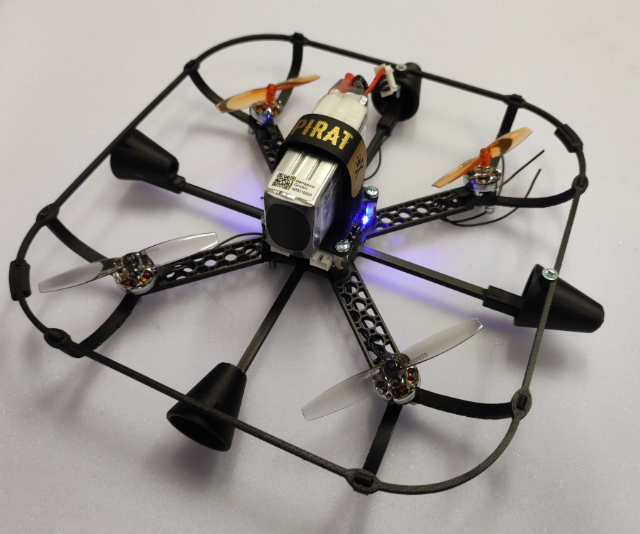
\includegraphics[width=\linewidth]{8-Etat_de_art/travaux_preli/pic/crazyflie_structure.PNG} \caption{UAV eSWARM} \label{fig:crazyflie_struct} \vspace{-0.5cm} \end{wrapfigure}

Le projet eSWARM a été initié en 2023 par Sylvain Boegeat, qui, lors d'un stage de deux mois, a développé une structure d'accroche à fixer sur des drones de type Crazyflie \cite{boegeat_rapport_2023}. Par la suite, dans le cadre du projet de recherche technologique (PRT) à l'INSA Strasbourg, il a collaboré avec Augustin Bonnel pour améliorer le système \cite{boegeat_rapport_2023-1}.

La production finale obtenue après ces deux projets est illustrée en Fig. \ref{fig:crazyflie_struct}. Le système d'accroche est constitué de structures coniques imprimées en 3D, chacune intégrant un aimant, permettant la fixation à un autre drone équipé de la même structure. Ce mécanisme garantit un degré de liberté (roulis ou tangage) entre deux drones connectés.

Un autre objectif du PRT était la rédaction d'une première documentation sur l'utilisation des drones Crazyflie  ainsi que sur le logiciel de Motion Capture \textit{Motive}, utilisé pour estimer la position des drones dans l'espace. Une mise en vol de deux drones connectés est visible \href{https://www.youtube.com/shorts/q4ulvEUqU14}{\underline{ici}}.

\subsection{Travaux d'Augustin Bonnel (2024)} \label{partie:aug_bon}

Les travaux décrits ici ont été réalisés dans le cadre du projet de fin d'études d'Augustin Bonnel, en 2024 \cite{bonnel_modeling_2024}. Durant ses six mois de stage, il s'est concentré sur la modélisation du système, notamment sur le modèle de deux quadricoptères assemblés.

Il a d'abord rappelé le modèle d'un unique quadricoptère, en se basant sur le cours \cite{gangloff_mooc_2023}. Puis, il a entrepris la modélisation et la commande d'un système composé de deux drones, pouvant être assimilé à un octocoptère. Son approche repose sur l'utilisation d'une matrice de distribution permettant de convertir la commande de l'octocoptère en commandes individuelles pour chaque drone. Cette méthode permet de découpler le contrôle global de la structure du contrôle local de chaque UAV. Chaque drone applique alors les commandes adaptées à sa position et à la configuration globale du système.

Un modèle non linéaire a été initialement développé, puis un équivalent simplifié a été obtenu en linéarisant le système autour d'un point d'équilibre. Ce modèle reste valide uniquement si la structure évolue à proximité de ce point. Augustin a ensuite identifié les tâches restantes, comme le dimensionnement et le réglage du correcteur permettant de contrôler le système.